\documentclass{standalone}

\usepackage{tikz}
\usetikzlibrary {arrows.meta}

\usepackage{amsmath}

\begin{document}
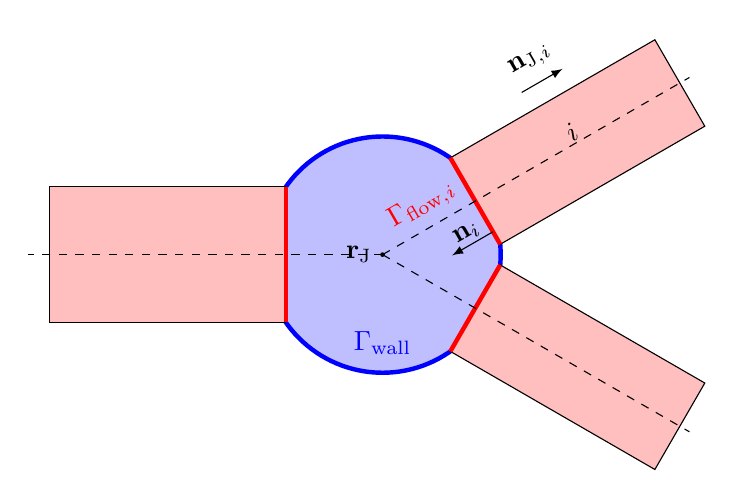
\begin{tikzpicture}[scale=3]

\newcommand{\pointradius}{0.01}
\newcommand{\labelspace}{0.1}
\newcommand{\arrowlength}{0.2}
\newcommand{\juncradius}{0.5}
\newcommand{\channeloneangle}{30}
\newcommand{\channeltwoangle}{180}
\newcommand{\channelthreeangle}{330}
\newcommand{\channeloneanglewidth}{50}
\newcommand{\channeltwoanglewidth}{70}
\newcommand{\channelthreeanglewidth}{50}
\newcommand{\channellength}{1}

\coordinate (pJ) at (0,0);

% junction
\draw[blue, ultra thick, fill=blue!25!white] (pJ) circle (\juncradius);
\fill (pJ) circle (\pointradius);
\node at (-\labelspace, 0) {$\mathbf{r}_\text{J}$};
\node[blue] at (0, {-0.75 * \juncradius}) {$\Gamma_{\text{wall}}$};

% channel i (upper right)
\draw[fill=red!25!white, rotate around={\channeloneangle:(pJ)}]
  ({\juncradius * cos(\channeloneanglewidth / 2)}, {\juncradius * sin(\channeloneanglewidth / 2)})
  rectangle
  ({\juncradius * cos(\channeloneanglewidth / 2) + \channellength}, {-\juncradius * sin(\channeloneanglewidth / 2)});
\draw[red, ultra thick, rotate around={\channeloneangle:(pJ)}]
  ({\juncradius * cos(\channeloneanglewidth / 2)}, {\juncradius * sin(\channeloneanglewidth / 2)}) --
  ({\juncradius * cos(\channeloneanglewidth / 2)}, {-\juncradius * sin(\channeloneanglewidth / 2)});
\draw[dashed] (pJ) -- ({(\channellength + \juncradius) * cos(\channeloneangle)},
  {(\channellength + \juncradius) * sin(\channeloneangle)});
\node[red, rotate around={\channeloneangle:(pJ)}] at ({0.5 * \juncradius}, 0.1) {$\Gamma_{\text{flow},i}$};
\node[rotate around={\channeloneangle:(pJ)}]
  at ({\juncradius * cos(\channeloneanglewidth / 2) + \channellength / 2}, 0.05) {$i$};
\node[rotate around={\channeloneangle:(pJ)}]
  at ({\juncradius * cos(\channeloneanglewidth / 2) - \arrowlength / 2}, -0.1) {$\mathbf{n}_i$};
\draw[-{latex[length=1.5mm, width=1mm]}, rotate around={\channeloneangle:(pJ)}]
  ({\juncradius * cos(\channeloneanglewidth / 2)}, -0.15)
  -- ({\juncradius * cos(\channeloneanglewidth / 2) - \arrowlength}, -0.15);
\node[rotate around={\channeloneangle:(pJ)}]
  at ({\juncradius * cos(\channeloneanglewidth / 2) + \channellength * 0.5}, 0.4) {$\mathbf{n}_{\text{J},i}$};
\draw[-{latex[length=1.5mm, width=1mm]}, rotate around={\channeloneangle:(pJ)}]
  ({\juncradius * cos(\channeloneanglewidth / 2) + \channellength * 0.5 - \arrowlength / 2}, 0.3)
  -- ({\juncradius * cos(\channeloneanglewidth / 2) + \channellength * 0.5 + \arrowlength / 2}, 0.3);

% channel k (left)
\draw[fill=red!25!white, rotate around={\channeltwoangle:(pJ)}]
  ({\juncradius * cos(\channeltwoanglewidth / 2)}, {\juncradius * sin(\channeltwoanglewidth / 2)})
  rectangle
  ({\juncradius * cos(\channeltwoanglewidth / 2) + \channellength}, {-\juncradius * sin(\channeltwoanglewidth / 2)});
\draw[red, ultra thick, rotate around={\channeltwoangle:(pJ)}]
  ({\juncradius * cos(\channeltwoanglewidth / 2)}, {\juncradius * sin(\channeltwoanglewidth / 2)}) --
  ({\juncradius * cos(\channeltwoanglewidth / 2)}, {-\juncradius * sin(\channeltwoanglewidth / 2)});
\draw[dashed] (pJ) -- ({(\channellength + \juncradius) * cos(\channeltwoangle)},
  {(\channellength + \juncradius) * sin(\channeltwoangle)});

% channel m (lower right)
\draw[fill=red!25!white, rotate around={\channelthreeangle:(pJ)}]
  ({\juncradius * cos(\channelthreeanglewidth / 2)}, {\juncradius * sin(\channelthreeanglewidth / 2)})
  rectangle
  ({\juncradius * cos(\channelthreeanglewidth / 2) + \channellength}, {-\juncradius * sin(\channelthreeanglewidth / 2)});
\draw[red, ultra thick, rotate around={\channelthreeangle:(pJ)}]
  ({\juncradius * cos(\channelthreeanglewidth / 2)}, {\juncradius * sin(\channelthreeanglewidth / 2)}) --
  ({\juncradius * cos(\channelthreeanglewidth / 2)}, {-\juncradius * sin(\channelthreeanglewidth / 2)});
\draw[dashed] (pJ) -- ({(\channellength + \juncradius) * cos(\channelthreeangle)},
  {(\channellength + \juncradius) * sin(\channelthreeangle)});

\end{tikzpicture}
\end{document}
